\documentclass[11pt]{article}
\usepackage{latexsym}
\usepackage{amsmath}
\usepackage{amssymb}
\usepackage{amsthm}
\usepackage{epsfig}
\usepackage[tight]{subfigure}
\usepackage{subcaption}
\usepackage{amsmath}

\DeclareMathOperator*{\minimize}{min}
\DeclareMathOperator*{\maximize}{max}

\usepackage{algorithm}
 %on linux you may need to run sudo apt-get install texlive-full to install algorithm.sys
\usepackage{algorithmic}
\renewcommand{\algorithmiccomment}[1]{\hfill //~#1\normalsize}
\usepackage{verbatim}

\newcommand{\handout}[5]{
  \noindent
  \begin{center}
  \framebox{
    \vbox{
      \hbox to 5.78in { {#1} \hfill #2 }
      \vspace{4mm}
      \hbox to 5.78in { {\Large \hfill #5  \hfill} }
      \vspace{2mm}
      \hbox to 5.78in { {\em #3 \hfill #4} }
    }
  }
  \end{center}
  \vspace*{4mm}
}

\newcommand{\lecture}[5]{\handout{#1}{#2}{#3}{#4}{#5}}
\newcommand{\collision}[0]{\mathrm{collision}}
\newcommand{\nocollision}[0]{\overline{\collision}}

\newcommand*{\QED}{\hfill\ensuremath{\square}}

\newtheorem{theorem}{Theorem}
\newtheorem{corollary}[theorem]{Corollary}
\newtheorem{lemma}[theorem]{Lemma}
\newtheorem{observation}[theorem]{Observation}
\newtheorem{proposition}[theorem]{Proposition}
\newtheorem{definition}[theorem]{Definition}
\newtheorem{claim}[theorem]{Claim}
\newtheorem{fact}[theorem]{Fact}
\newtheorem{assumption}[theorem]{Assumption}
\newtheorem{note}[theorem]{Note}

% 1-inch margins, from fullpage.sty by H.Partl, Version 2, Dec. 15, 1988.
\topmargin 0pt
\advance \topmargin by -\headheight
\advance \topmargin by -\headsep
\textheight 8.9in
\oddsidemargin 0pt
\evensidemargin \oddsidemargin
\marginparwidth 0.5in
\textwidth 6.5in

\parindent 0in
\parskip 1.5ex
%\renewcommand{\baselinestretch}{1.25}

\begin{document}

\lecture{Statistical Techniques in Robotics (16-831, S20)}{Lecture \#04
  (Monday, January 13)}{Lecturer: Kris Kitani}{Scribes: Jeet Kanjani, Shubham Gupta}{Online Techniques for Support Vector Machines (SVMs)}

\section{Review}
    \begin{flushleft}
    In the last lectures, we studied the concepts of Online Gradient Descent (OGD) and Stochastic Gradient Descent (SGD) and how it is applied to solve the online learning problems. In the next sections, we first recap the SGD algorithm, build the necessary mathematical fundamentals and finally use them to solve the support vector machines. We finally draw comparisons between the perceptron algorithm and support vector machines.
    
    In supervised learning, we have a separate training and test set where the algorithm learns using the examples in the training set and validates the performance on the test set. Online learning however has a single dataset that comes in the form of the data stream. We predict on this data and simultaneously use it for training as well. This can be viewed as an interleaving of training and test set in the supervised setting. In essence, online learning interweaves the training and testing steps.
\end{flushleft}
    \begin{figure}[h!]
    \centering
    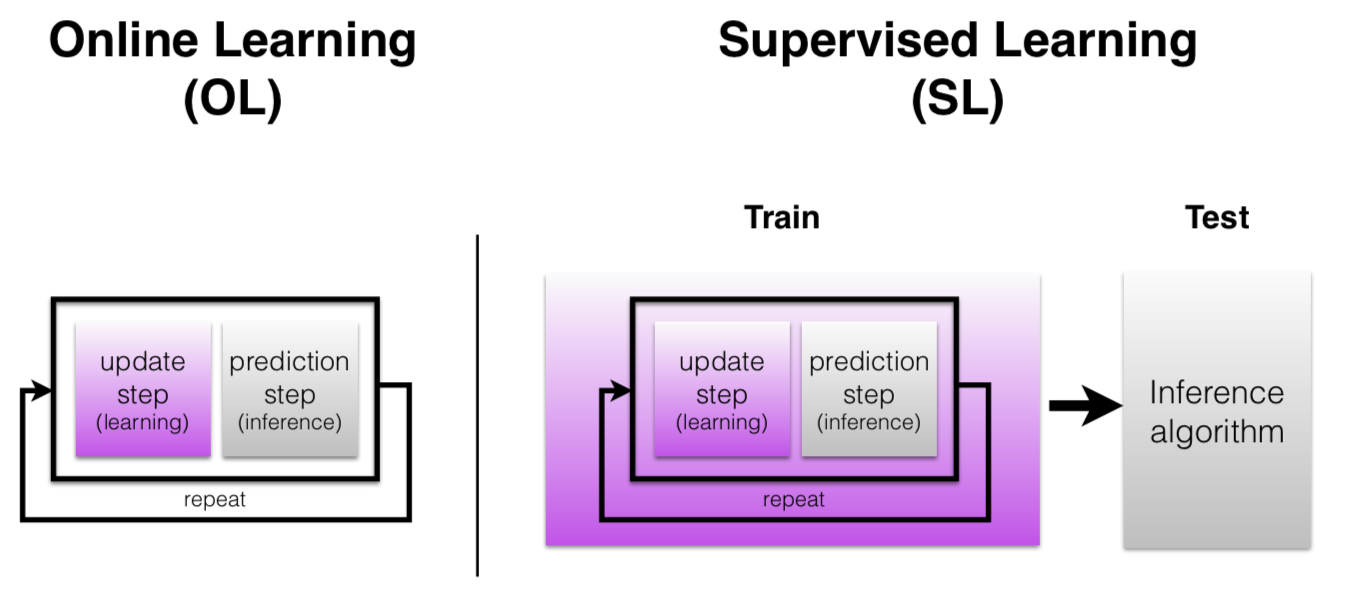
\includegraphics[scale=0.3]{images/online_supervised.png}
    \caption{Online Learning v/s Supervised Learning}
    \end{figure}


%This section serves as a review of the previous lecture and any other context required to frame the content of the current lecture. 

%You may format the scribes in any way you like, aside from changing font style, size and page format. Please use subsections and paragraphs to increase the readability of your notes.

%Length requirement 1-2 pages.
        
\subsection{Online (Projected Sub-) Gradient descent}
Recall, the regularization and the loss function as:

	\begin{equation}
	\begin{aligned}
    &\psi(w) = \frac{1}{2\eta} ||w||^2 \\
	&f(w) = \langle w, \theta \rangle
    \end{aligned}
	\end{equation}
	
	\begin{algorithm}
	\caption{Online SUB-GRADIENT DESCENT}
    \begin{algorithmic}[1]
    \FOR{t=1,2,3...T}
    \STATE $\theta^{(t+1)}  = \theta^{(t)} -\eta z^{(t)} $ \COMMENT{with some assumption on the magnitude of the sub gradient}
    \STATE $w^{(t+1)} = -\eta \theta^{(t+1)}$ \COMMENT{Mirror projection}
    \ENDFOR
    \end{algorithmic}
	\end{algorithm}


	\begin{algorithm}
	\caption{Online PROJECTED SUB-GRADIENT DESCENT}
    \begin{algorithmic}[1]
    \FOR{t=1,2,3...T}
    \STATE $\theta^{(t+1)}  = \theta^{(t)} -\eta z^{(t)} $ \COMMENT{Dual paramter update}
    \STATE $w^{(t+1)} = \prod_{\theta \to S}-\eta \theta^{(t+1)}$ \COMMENT{Mirror projection}
    \ENDFOR
    \end{algorithmic}
	\end{algorithm}

\section{Summary}

%\section*{References}
%Include your references here. Please cite any resources you found useful.	
%Populate the refs.bib file or list your references manually. Be consistent in formatting!
\subsection{Hyperplane}
A hyperplane is a plane that divides the n-dimensional data points into two components. It is called a line in 2D and a plane in the case of 3D.
\subsubsection{Distance of line from the origin}

	For an arbitrary line wx + b, the distance of the origin to the line is given by:
	
	\begin{figure}[h!]
    \centering
    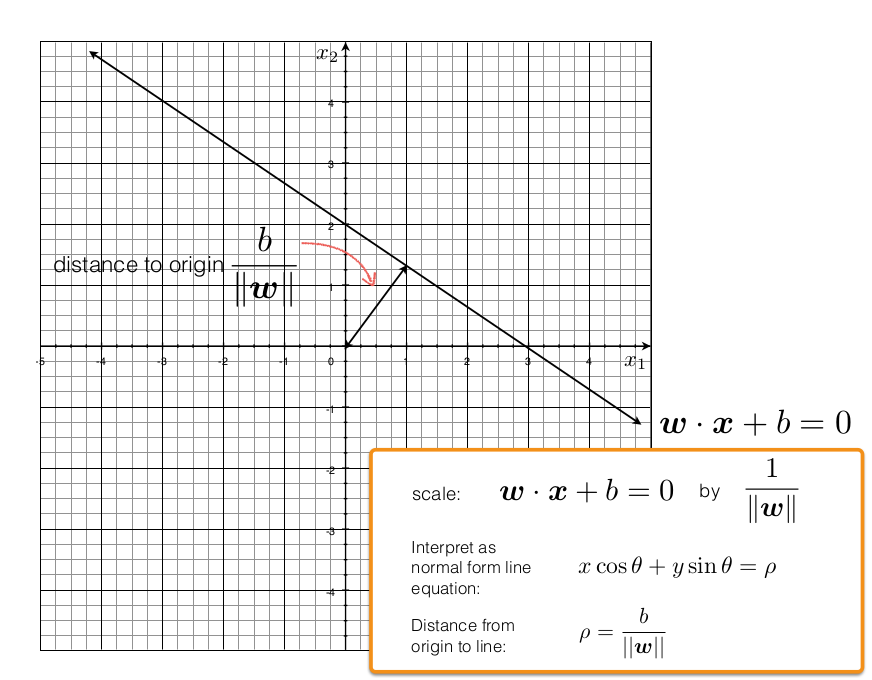
\includegraphics[scale=0.3]{images/distance_to_origin.png}
    \caption{Distance of line from the origin}
    \label{fig:method}
    \end{figure}

Distance of a hyperplane y = $w\cdot x_i$ + b where w \in R^N$ from the origin is also given by $\frac{b}{||w||}$.
\subsubsection{Margin}
  The distance between two parallel hyperplanes generated by shifting the planes by one in and opposite to the direction of w is given by: 

	\begin{equation}
	\begin{aligned}
	&M = \frac{(1 - b)}{(|W|)} - \frac{(-1 - b)}{(|W|)} \\
	&M = \frac{2}{|W|}
	\end{aligned}
	\end{equation}
	
	\begin{figure}[h!]
    \centering
    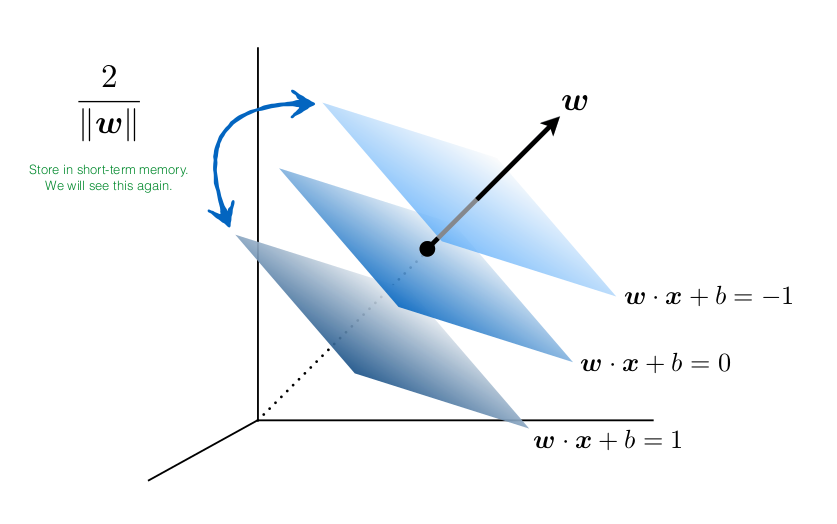
\includegraphics[scale=0.3]{images/margin.png}
    \caption{Margin of the hyperplane}
    \label{fig:method}
    \end{figure}
	


The margin of the hyperplane is the minimum distance between the hyperplane and the closest data point. 

\subsection{Optimal margin}
An optimal hyperplane is the one which maximizes this margin. In canonical form it is given by\cite{bishop}:

	\begin{equation}
	\begin{aligned}
	&\max_{w} \left( \frac{2}{||w||}\right)\\
	\\
	\text{subject to, }  w.x_i + b \text{   }
    &\begin{Bmatrix}
    \geq +1 \text{ if } y_i= +1 \\
    \leq -1 \text{ if } y_i = -1 
    \end{Bmatrix}
    \text{  for i = 1,...,N}
	\end{aligned}
	\end{equation}

	\begin{figure}[h!]
    \centering
    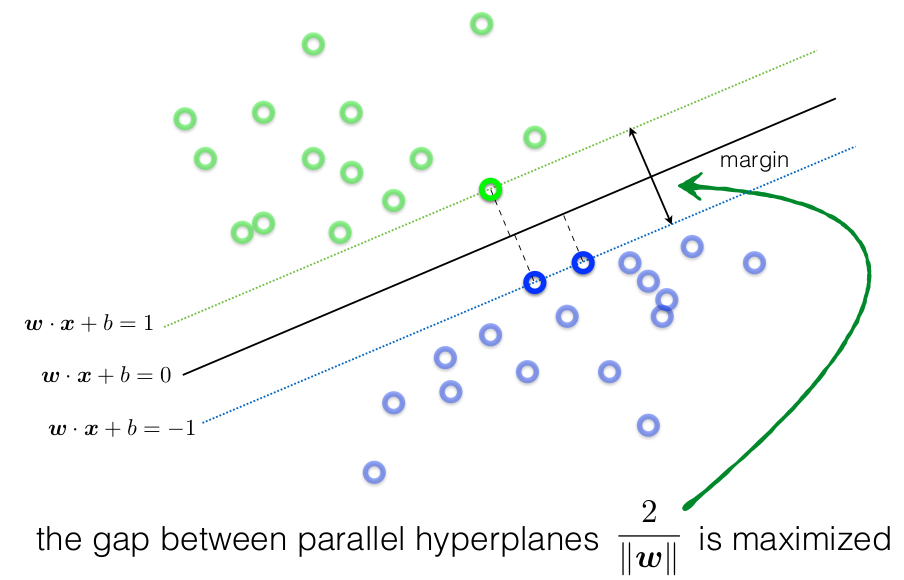
\includegraphics[scale=0.4]{images/max_margin.png}
    \caption{Max Margin of the hyperplane}
    \label{fig:method}
    \end{figure}
	

Since the l2 optimizations are much more stable than the l1 optimization, the above equation could be written as\cite{ankit}:

	\begin{equation}
	\begin{aligned}
	&\min_{w} \left(||w||^2\right)\\ \\
	\text{subject to, }  y_i(&w.x_i + b) \geq 1 \text{   }
    \text{  for i = 1,...,N}
	\end{aligned}
	\end{equation}

This notational trick of $y_i(w.x_i + b)$ only works when doing binary classification. The loss function is changed to a quadratic such that we can make a connection to the online convex optimization. This is also called the \textbf{primal} form of a linear SVM. The optimization is a convex quadratic programming problem.  

\subsection{Soft Margin SVM}
When the data is not linearly separable, the soft margin allows the SVM to make a certain number of mistakes and keep the margin as wide as possible so that other points can still be classified correctly\cite{rishabh}. To achieve this, some relaxation is put on the hard constraint  $y_i(w.x_i + b)$ by introducing slack variable $\xi$:

 	\begin{equation}
	\begin{aligned}
	&\min_{w, \xi} \left(||w||^2 + C\sum_i \xi_i\right)\\
	\text{subject to, }  &y_i(w\cdot x_i + b) \geq 1 - \xi_i \text{   }
    \text{  for i = 1,...,N, }\xi_i > 0
	\end{aligned}
	\end{equation}
	here C is a regularization hyperparameter that decides the trade-off between maximizing the margni and minimizing the mistakes. When C is small, classification mistakes are given less importance and focus is more on maximizing the margin. Whereas when C is large, emphasis is on avoiding misclassification at the expense of keeping the margin small. Since, we have a linear objective with a quadratic regularizer, we can use stochastic gradient descent to solve this. On merging the linear constraints into the objective function, we get:
	
	\begin{equation}
	\begin{aligned}
	\min_w \left(\frac{\lambda}{2}||w||^2 + \frac{1}{M} \sum_{m=1}^{M} (1 - y_mw^Tx_m) \right)
	\end{aligned}
	\end{equation}
	
	However, in our objective function, we are interested in the points which are incorrectly classified and the weakly correct ones (ignoring the very correct ones). 
	\begin{figure}[h!]
    \centering
    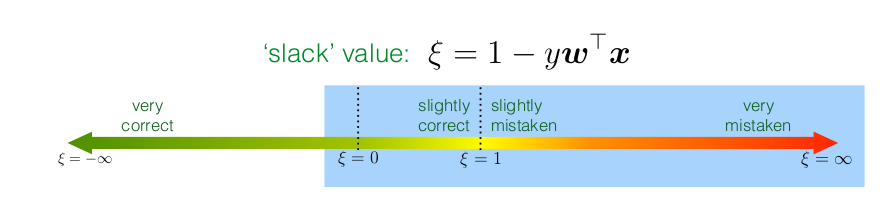
\includegraphics[scale=0.4]{images/xi.png}
    \caption{points in slightly correct, slightly mistaken and very mistaken are the ones objective function should be optimized on.}
    \label{fig:method}
    \end{figure}
    
    The way to achieve this is Hinge Loss:
	
    \begin{equation}
	\begin{aligned}
	\min_w \left(\frac{\lambda}{2}||w||^2 + \frac{1}{M} \sum_{m=1}^{M} \max \{0,1 - y_mw^Tx_m\} \right)
	\end{aligned}
	\end{equation}
	
	
	Now that we have a convex but not differentiable function (due to the hinge), we can use sub-gradient descent to optimize this. 
\subsection{Sub-gradients}
The gradient descent algorithm discussed above requires the loss function to be differentiable. To use it for this class of non-differentiable convex functions, we have to do certain modifications. We achieve this by introducing the concept of subgradients. Subgradient refers to the possible set of gradients for a non-differentiable convex function. 
    \begin{figure}[h!]
    \centering
    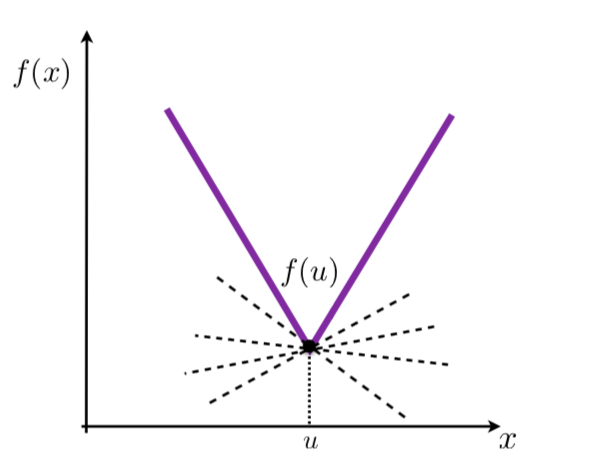
\includegraphics[scale=0.3]{images/sub_gradients.png}
    \caption{Multiple gradients (sub-gradients) at $x=u$ for $f(x)$}
    \end{figure}
\newline Consider the function given in the above image. We can consider any of the possible gradients at point $x=u$ for the function $f(u)$. We call this set of possible gradients at point $x=u$ as sub-gradients for $f(u)$.
\subsection{Online Sub-gradient Descent}
Online sub-gradient descent is an algorithm used to assign gradient to a non-differentiable convex function. The algorithm uses any one of all the available sub-gradients for the non-differentiable points. Thus, we can use sub-gradient descent for soft-margin SVM optimization.
\newline Recall soft margin SVM loss is given by
\[ \min_w \left(\frac{\lambda}{2}||w||^2 + \frac{1}{M} \sum_{m=1}^{M} \max \{0,1 - y_mw^Tx_m\} \right) \]
Here, the second term ($\frac{1}{M} \sum_{m=1}^{M} \max \{0,1 - y_mw^Tx_m\}$) is hinge loss (non-differentiable). 

\begin{figure}[h!]
\centering
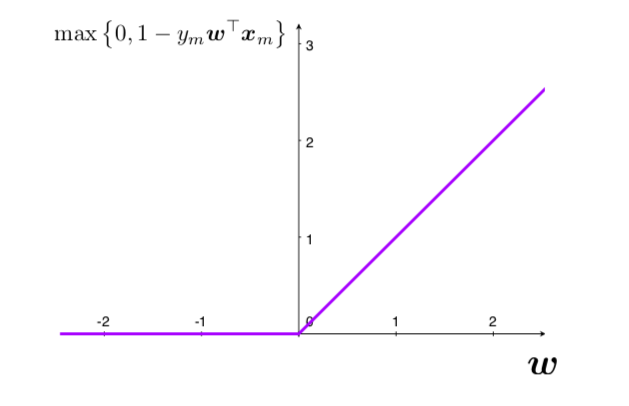
\includegraphics[scale=0.5]{images/hinge.png}
\caption{Hinge Loss}
\end{figure}
We consider 2 possible sub-gradients to optimize this loss function.
\[
    z_m =
    \begin{cases}
        0 & \text{if $y_mw^Tx_m \geq 1$,}\\
        -y_mx_m & \text{otherwise}
    \end{cases}
\]

\textbf{Case 1:}
Note that when $y_mw^Tx_m$ is greater than 1, it means that the point is correctly classified by the algorithm and far from the margin. We consider the hinge loss gradient to be zero in this case.
\newline\textbf{Case 2} 
When $y_mw^Tx_m$ is less than 1, it means that we have either incorrect classification, or the point lies within the margin. We consider the gradient of loss to be $-y_mx_m$ in this case.

\subsection{Soft Margin SVM Optimization using Online Sub-gradient Descent}
Using the gradient derived for hinge loss in the previous section, we can write an update rule for the weights. Below is the pseudo code for the algorithm
	\textbf{Pseudo Code:}
	\begin{algorithm}
	\caption{SoftSVM(\lambda)}
    \begin{algorithmic}[1]
    \STATE $\theta^{(1)} \leftarrow 0 \in R^N$ \COMMENT{Written in the \textbf{OMD} format}
    \FOR{t=1,2,3...T}
    \STATE $x_d, y_d \sim D$ \COMMENT{Receive sample from environment}
    \STATE $\theta^{(t)} = \theta^{(t-1)} + y_dx_d.1[y_d(w^{(t)}.x_d) < 1]$ \COMMENT{Dual parameter update}
    \STATE $w^{(t+1)} \leftarrow \frac{1}{\lambda (t+1)}\theta^{(t)}$ \COMMENT{Mirror Projection}
    \ENDFOR
    \end{algorithmic}
	\end{algorithm}
\subsection{Comparison with Perceptron}
Recall that the perceptron algorithm in an online setting is given as follows
\newline\textbf{Pseudo Code:}
\begin{algorithm}[H]
\caption{Perceptron}
\begin{algorithmic}[1]
\STATE $w^{(1)} \leftarrow 0$ \COMMENT{Written in the \textbf{OMD} format}
\FOR{t=1,2,3...T}
\STATE RECEIVE $x^{(t)} \in R^N$ \COMMENT{Receive input from environment}
\STATE $\hat{y}^{t} = sign(w^{(t)}\cdot x^{(t)})$
\STATE RECEIVE $y^{(t)} \in \{1,-1\}$ \COMMENT{Get the Target }
\STATE $w^{(t+1)} = w^{(t)} + y^tx^{(t)}.1[y^{(t)} \neq \hat{y}^{(t)}]$ \COMMENT{Weight Update}
\ENDFOR
\end{algorithmic}
\end{algorithm}
Putting these side by side for comparison, we can see that only 2 lines (highlighted) differ in both the algorithms.
\begin{figure}[H]
\centering
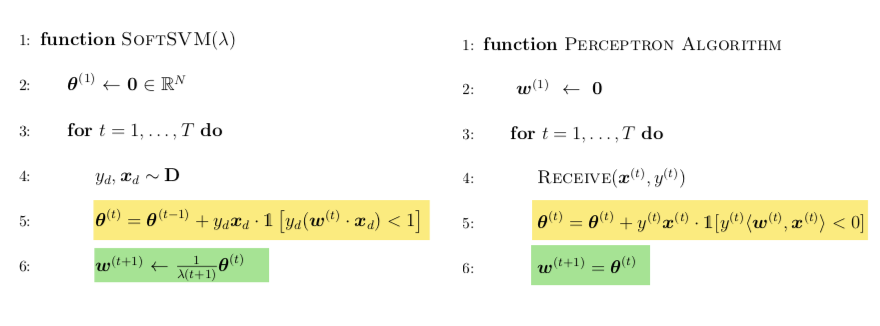
\includegraphics[scale=0.5]{images/comp_percep.png}
\caption{Comparison between SoftSVM and Perceptron Algorithm}
\end{figure}
We can observe that both SVM and perceptron are almost similar - both have piece-wise linear loss with quadratic regularization. Both use similar dual parameter updates and share the same mirror function. But there are 2 key differences.

\begin{enumerate}
    \item SVM uses a soft margin of 1 in line 5 whereas, perceptron doesn't have a concept of margin. All perceptron cares about whether all labels are correctly classified or not.
    \item The weight update rule has a multiplication factor in the SVM whereas for perceptron there is no such factor. This is due to the slack variable C present in the SVM objective function. 
\end{enumerate}

{
\bibliography{refs}
\bibliographystyle{abbrv}
\begin{thebibliography}{9}
    \bibitem{bishop} 
    C Bishop, Pattern Recognition and Machine Learning, 2005
    \bibitem{rishabh} 
    R Mishra, SVM soft margin formulation and kernel trick\\
    [\textit{https://towardsdatascience.com/support-vector-machines-soft-margin-formulation-and-kernel-trick-4c9729dc8efe}]
    \bibitem{ankit} 
    MlMathIO Math behind support vector machine\\
    [\textit{https://medium.com/@ankitnitjsr13/math-behind-support-vector-machine-svm-5e7376d0ee4d}]
\end{thebibliography}

}


%\section{Appendix}
%This section provides any relevant background material that was not covered in the lectures but was found to be useful for understanding the material. 
%For example, derivations, theory underlying techniques employed, etc. 

%Additionally, this section can summarize applications or extensions of these techniques found in the literature. 

\end{document} % Done!


